% オリジナルの tex 環境では 4-16 行をコメントアウトして,
% 20-61 行のコメントを元に戻して下さい.
%--------------------------------------------------------
\documentclass[twocolumn,10pt]{jarticle}
\usepackage{tc2016_utf}
\usepackage[dvipdfmx]{graphicx,color}
\usepackage[fleqn]{amsmath}
\usepackage{algorithm,algorithmic}
\usepackage{amssymb,epsfig}
\usepackage{ascmac}

\usepackage{url}
\usepackage{bm}
\usepackage{ascmac}
\usepackage{pifont}
%\usepackage{multirow}
\usepackage{enumerate}
%\usepackage{cases}
\usepackage{type1cm}
\usepackage{here}
\usepackage{secdot}
\sectiondot{subsection}
\sectiondot{subsubsection}

\DeclareRelationFont{JY1}{mc}{it}{}{OT1}{cmr}{it}{}
\DeclareRelationFont{JT1}{mc}{it}{}{OT1}{cmr}{it}{}
\DeclareFontShape{JY1}{mc}{m}{it}{<5> <6> <7> <8> <9> <10> sgen*min
    <10.95><12><14.4><17.28><20.74><24.88> min10
    <-> min10}{}
\DeclareFontShape{JT1}{mc}{m}{it}{<5> <6> <7> <8> <9> <10> sgen*tmin
    <10.95><12><14.4><17.28><20.74><24.88> tmin10
    <-> tmin10}{}
\DeclareRelationFont{JY1}{mc}{sl}{}{OT1}{cmr}{sl}{}
\DeclareRelationFont{JT1}{mc}{sl}{}{OT1}{cmr}{sl}{}
\DeclareFontShape{JY1}{mc}{m}{sl}{<5> <6> <7> <8> <9> <10> sgen*min
    <10.95><12><14.4><17.28><20.74><24.88> min10
    <-> min10}{}
\DeclareFontShape{JT1}{mc}{m}{sl}{<5> <6> <7> <8> <9> <10> sgen*tmin
    <10.95><12><14.4><17.28><20.74><24.88> tmin10
    <-> tmin10}{}
\DeclareRelationFont{JY1}{mc}{sc}{}{OT1}{cmr}{sc}{}
\DeclareRelationFont{JT1}{mc}{sc}{}{OT1}{cmr}{sc}{}
\DeclareFontShape{JY1}{mc}{m}{sc}{<5> <6> <7> <8> <9> <10> sgen*min
    <10.95><12><14.4><17.28><20.74><24.88> min10
    <-> min10}{}
\DeclareFontShape{JT1}{mc}{m}{sc}{<5> <6> <7> <8> <9> <10> sgen*tmin
    <10.95><12><14.4><17.28><20.74><24.88> tmin10
    <-> tmin10}{}
\DeclareRelationFont{JY1}{gt}{it}{}{OT1}{cmbx}{it}{}
\DeclareRelationFont{JT1}{gt}{it}{}{OT1}{cmbx}{it}{}
\DeclareFontShape{JY1}{mc}{bx}{it}{<5> <6> <7> <8> <9> <10> sgen*goth
    <10.95><12><14.4><17.28><20.74><24.88> goth10
    <-> goth10}{}
\DeclareFontShape{JT1}{mc}{bx}{it}{<5> <6> <7> <8> <9> <10> sgen*tgoth
    <10.95><12><14.4><17.28><20.74><24.88> tgoth10
    <-> tgoth10}{}
\DeclareRelationFont{JY1}{gt}{sl}{}{OT1}{cmbx}{sl}{}
\DeclareRelationFont{JT1}{gt}{sl}{}{OT1}{cmbx}{sl}{}
\DeclareFontShape{JY1}{mc}{bx}{sl}{<5> <6> <7> <8> <9> <10> sgen*goth
    <10.95><12><14.4><17.28><20.74><24.88> goth10
    <-> goth10}{}
\DeclareFontShape{JT1}{mc}{bx}{sl}{<5> <6> <7> <8> <9> <10> sgen*tgoth
    <10.95><12><14.4><17.28><20.74><24.88> tgoth10
    <-> tgoth10}{}
\DeclareRelationFont{JY1}{gt}{sc}{}{OT1}{cmbx}{sc}{}
\DeclareRelationFont{JT1}{gt}{sc}{}{OT1}{cmbx}{sc}{}
\DeclareFontShape{JY1}{mc}{bx}{sc}{<5> <6> <7> <8> <9> <10> sgen*goth
    <10.95><12><14.4><17.28><20.74><24.88> goth10
    <-> goth10}{}
\DeclareFontShape{JT1}{mc}{bx}{sc}{<5> <6> <7> <8> <9> <10> sgen*tgoth
    <10.95><12><14.4><17.28><20.74><24.88> tgoth10
    <-> tgoth10}{}
\DeclareRelationFont{JY1}{gt}{it}{}{OT1}{cmr}{it}{}
\DeclareRelationFont{JT1}{gt}{it}{}{OT1}{cmr}{it}{}
\DeclareFontShape{JY1}{gt}{m}{it}{<5> <6> <7> <8> <9> <10> sgen*goth
    <10.95><12><14.4><17.28><20.74><24.88> goth10
    <-> goth10}{}
\DeclareFontShape{JT1}{gt}{m}{it}{<5> <6> <7> <8> <9> <10> sgen*tgoth
    <10.95><12><14.4><17.28><20.74><24.88> tgoth10
    <-> tgoth10}{}
\endinput
%%%% end of jdummy.def

\def\vec#1{\mbox{\boldmath$#1$}}
\def\vector#1{\mbox{\boldmath $#1$}}

\newcommand{\argmax}{\mathop{\rm arg~max}\limits}
\newcommand{\argmin}{\mathop{\rm arg~min}\limits}
\newcommand{\umax}{\mathop{\rm max}\limits}

\def\R{{\Bbb R}}
\def\Z{{\Bbb Z}}

\renewcommand{\topfraction}{0.8}
\renewcommand{\bottomfraction}{0.8}
\renewcommand{\dbltopfraction}{0.8}
\renewcommand{\textfraction}{0.1}
\renewcommand{\floatpagefraction}{0.8}
\renewcommand{\dblfloatpagefraction}{0.8}
\setcounter{topnumber}{3}
\setcounter{bottomnumber}{3}
\setcounter{totalnumber}{3}
\title{\vspace{-20truemm}
{\normalsize \rightline{平成29年\ 12月\ 13日}}
{\large つくばチャレンジ 2017\\}
成果報告
\date{}
\vspace{-2truemm}}
%----------------------------------------
\author{西田研究室 M1 西尾 貴樹} %番号氏名
%--------------------------------------------------------
\begin{document}
\twocolumn[\maketitle]
%--------------------------------------------------------
%--------------------------------------------------------
%--------------------------------------------------------
% %#BIBTEX pbibtex document
% %
% % 計測自動制御学会システム・インテグレーション部門学術講演会2012原稿サンプルファイル
% %                                           October 4, 2012
% % Based on 計測自動制御学会システム・情報部門学術講演会2012原稿サンプルファイル
% %                                           April 28, 2012
% % Based on 第7回計測自動制御学会制御部門大会原稿サンプルファイル
% %                                           October 18, 2007
% % Based on 第5回計測自動制御学会制御部門大会原稿サンプルファイル
% %            近野敦 konno@space.mech.tohoku.ac.jp    March 05, 2005
% %
% % Based on Github : yoneken/SI2012_sampleTeX
% % https://github.com/yoneken/SI2012_sampleTeX
% % https://github.com/yoneken/si2012.sty

% \documentclass[10pt,a4paper]{jarticle}
% \usepackage{style/si2015}

% \usepackage{url}
% \usepackage[dvips]{graphicx}
% \usepackage[numbers,super,square]{natbib}
% \usepackage{mathpazo}
% \usepackage{color}
% \usepackage{graphicx}
% \usepackage{listings}
% \usepackage{amsmath,amssymb}
% \usepackage{bm}
% \usepackage[subrefformat=parens]{subcaption}
% % \makeatletter
% % \def\thefigure{\thesection.\arabic{figure}}
% % \@addtoreset{figure}{section}
% % \makeatother

% \begin{document}
% \title{九州工業大学\\CIR-KIT B による独立二輪駆動型自律ロボットの開発と\\つくばチャレンジへの取り組み}
% \author{○田中 良道 有田 裕太 森田 賢 西田 健(九州工業大学)}
% \engauthor{
%   ○Ryodo Tanaka, Yuta Arita,\\
%   Masaru Morita, and Takeshi Nishida \\(Kyushu Institute of Technology)
% }
% \pagestyle{empty}
% \maketitle\thispagestyle{empty}
%--------------------------------------------------------
%--------------------------------------------------------
%--------------------------------------------------------
\section{人物探索}
%--------------------------------------------------------
\subsection{概要}
%--------------------------------------------------------
特定人物の探索を行うために,我々はニューラルネットワークによる一般物体認識技術を活用した.一般物体認識とは,RGB 画像から人や車,犬などの物体のラベル(種類)と位置(矩形領域)を認識するものである.現在までに開発されている一般物体認識のためのニューラルネットワークは,その多くが大規模な構造を有する CNN (Convolutional Neural Network) で構成されているため,本稿では一般物体認識 CNN と呼ぶ.一般物体認識 CNN は膨大なデータセットを利用し強力な計算機で学習されたもので,高精度に一般物体の認識を行うことができる.しかし,特定の物体の認識を行う場合,データセットを自分で用意して大規模 CNN の学習をやり直す必要がある.つくばチャレンジの人物探索タスクでは特定の服装の人物を発見することが目標となるが,このタスクに一般物体認識 CNN での認識を適用するためには,特定人物の矩形領域を手作業で対応付けた膨大な画像データを用意する必要があった.我々はこの問題を解決するため,公開されている学習済みの一般物体認識 CNN に特定人物分類のためのモジュール型 CNN をカスケード接続することで,特定の人物の探索を行えるようにした.今回は,一般物体認識 CNN には Redmon らが 2016 年に公開した YOLOv2\cite{yolo} を用いた.
%--------------------------------------------------------
\subsection{YOLOv2 について}
%--------------------------------------------------------
YOLOv2 は,入力された画像に対して一般物体のラベルと矩形領域を同時に認識する CNN である.公開されている学習済みモデルでは,人や車,電子レンジなど,80 種類の物体を複数同時に認識できる.類似の一般物体認識 CNN として,Fast R-CNN\cite{fast_r-cnn} や SSD\cite{ssd} 等があるが,それらより YOLOv2 の方が高速かつ高精度な認識が可能なため,今回は YOLOv2 を利用することに決定した.
%--------------------------------------------------------
\subsection{人物探索の流れ}
%--------------------------------------------------------
%-------------------------------
\begin{figure}[t]
\centering
 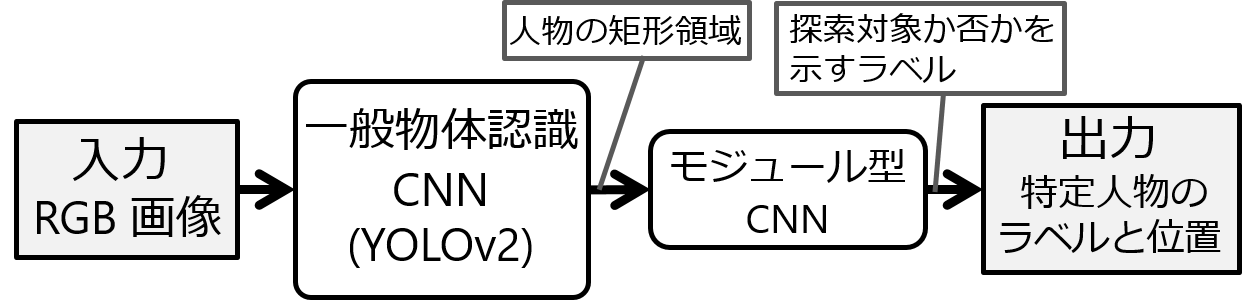
\includegraphics[scale=0.37]{fig/method.png}
 \caption{人物探索の流れ}
 \label{fig:method}
\end{figure}
%-------------------------------
Fig.\ref{fig:method} に我々が構成した人物探索のためのニューラルネットワークの構成を示す.はじめに,web カメラから得られるフレーム画像を YOLOv2 に入力し,「人物」の探索を行う.次に,そのフレーム画像から YOLOv2  が「人物」であると認識した矩形領域を切り出し,モジュール型 CNN に入力する.モジュール型 CNN は YOLOv2 が認識した「人物」が「探索対象の人物」か「その他の人物」かの判別(二値分類)を行う.つくばチャレンジでは探索対象の人物はオレンジ色もしくは青色のベストを着用するが,今回はその両方をまとめて「探索対象」と認識させることにした.この手法で学習が必要なニューラルネットワークは二値分類を行うモジュール型 CNN のみである.そのため,データセットは探索対象の人物およびその他の人物画像と探索対象か否かのラベルだけで済み,人物領域の矩形の座標データを付加する必要が無くなる.また,モジュール型 CNN はクラス分類を行うシンプルな CNN のため,一般物体認識 CNN よりはるかに単純な構造で実現が可能である.
%--------------------------------------------------------
\subsection{開発環境}
%--------------------------------------------------------
人物探索を行うために用意した開発環境を Table.\ref{tb:env} に示す.Table.\ref{tb:env} の開発環境はデスクトップ PC における構成だが,ロボットに搭載したノート PC も同等の性能を持つものを使用した.
%-------------------------------
\begin{table}[b]
 \begin{center}
  \caption{開発環境}
  \begin{tabular}{|c|c|} \hline
   項目 & 型式およびバージョン \\ \hline \hline
   OS & ubuntu 14.04 LTS \\ \hline
   CPU & intel core i7 6700 \\ \hline
   システムメモリ & 8GB \\ \hline
   GPU & NVIDIA GTX 1070 \\ \hline
   GPU ドライバ & CUDA 8.0 V8.0.44 \\ \hline
   プログラミング言語 & Python 2.7.6 \\ \hline
   NN フレームワーク & Chainer 1.18.0 \\ \hline
   画像処理ライブラリ & OpenCV 2.4.8 \\ \hline
   web カメラ & Logicool c930e \\ \hline
  \end{tabular}
  \label{tb:env}
 \end{center}
\end{table}
%-------------------------------
%--------------------------------------------------------
\subsection{データセットの作成}
%--------------------------------------------------------
データセットの作成方法としては,画像の合成による方法と,動画からの人物領域の切り出しによる方法の 2 つを利用した.さらに,画像の回転や反転,コントラスト調整などのデータの水増しを行い,最終的に探索対象人物の画像を 220832 枚,その他の人物の画像を 206672 枚,合計 427504 枚の画像を用意した.なお,動画からの人物領域の切り出しには YOLOv2 を用いた.データセットの一部を Fig.\ref{fig:dataset} に示す.
%-------------------------------
\begin{figure}[t]
\begin{center}
\subfloat[探索対象]{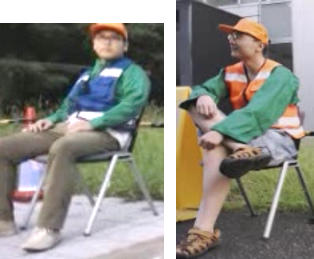
\includegraphics[scale=0.65]{fig/target.png}}
\hspace{0.7cm}
\subfloat[その他]{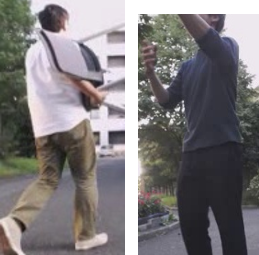
\includegraphics[scale=0.65]{fig/others.png}}
\caption{データセットの一部}
\label{fig:dataset}
\end{center}
\end{figure}
%-------------------------------
%--------------------------------------------------------
\subsection{モジュール型 CNN の学習}
%--------------------------------------------------------
モジュール型 CNN の構造を Fig.\ref{fig:module_cnn} に示す.Fig.\ref{fig:module_cnn} の CNN は,クラス分類に用いられる一般的な CNN の基本構造をそのまま利用したものである.
YOLOv2 の認識結果によって切り出された画像が,入力時に 50$\times$50 [pixel] の画像サイズに圧縮されている点に注意されたい.
Table.\ref{tb:params} にモジュール型 CNN の学習時に設定したパラメータを示す.未学習画像 1000 枚に対する正解率は 99.4 [\%] となった.
%-------------------------------
%-------------------------------
\begin{figure}[t]
\centering
 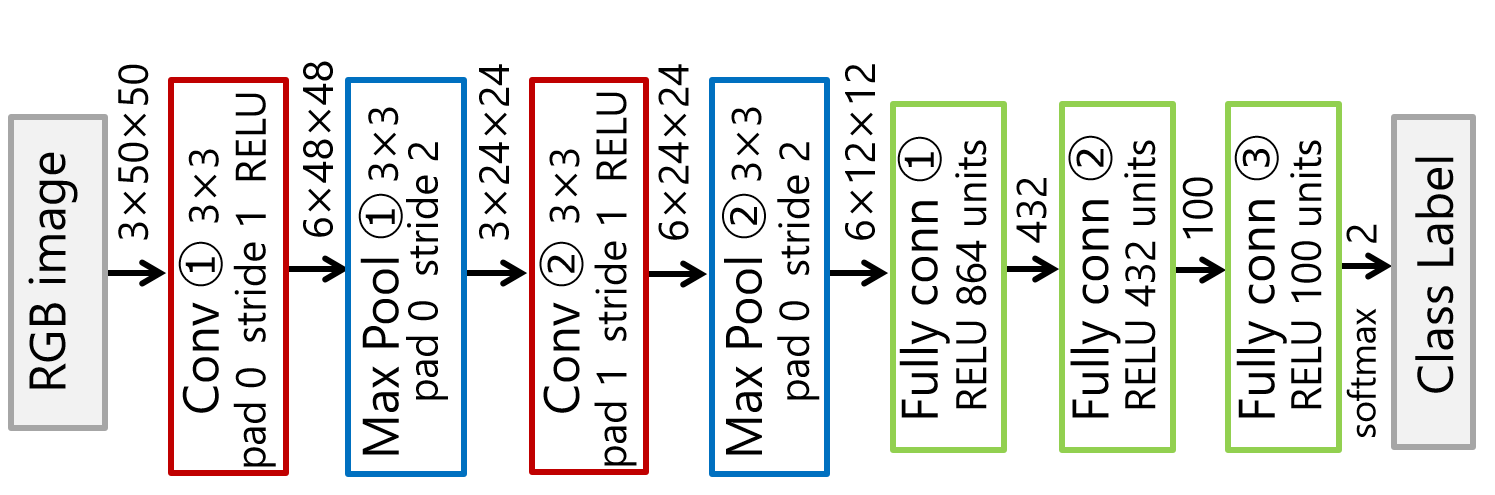
\includegraphics[scale=0.31]{fig/module_cnn.png}
 \caption{モジュール型 CNN の構造}
 \label{fig:module_cnn}
\end{figure}
%-------------------------------
\begin{table}[b]
 \begin{center}
  \caption{学習時のパラメータ}
  \begin{tabular}{|c|c|} \hline
   項目 & 設定値 \\ \hline \hline
   誤差関数 & Softmax cross entropy \\ \hline
   最適化アルゴリズム & Adam ($\alpha = 0.0001$) \\ \hline
   訓練用データ & 350000 セット\\ \hline
   確認用データ & 30000 セット \\ \hline
   ミニバッチサイズ & 50 \\ \hline
   繰り返し回数 & 10 \\ \hline
  \end{tabular}
  \label{tb:params}
 \end{center}
\end{table}
%-------------------------------
\begin{figure}[t]
\centering
 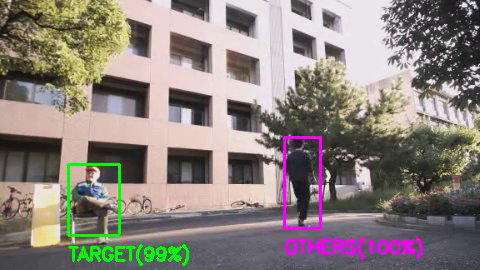
\includegraphics[scale=0.45]{fig/exp.png}
 \caption{実験の様子}
 \label{fig:exp}
\end{figure}
%-------------------------------
%--------------------------------------------------------
\subsection{実験結果と今後の課題}
%--------------------------------------------------------
一般物体認識 CNN である YOLOv2 と学習済みのモジュール型 CNN をカスケード接続し,カメラを繋いで実験を行った.実験の様子を Fig.\ref{fig:exp} に示す.GPU を用いるとほぼリアルタイムでの認識が可能になった.ただし,認識結果にちらつきが見られたり,誤認識が発生する場合があった.今回のつくばチャレンジではロボットへの実装は間に合わなかったが,来年は実装したいと考えている.それまでに,認識結果のちらつき防止,時系列情報を利用した認識後の物体のトラッキングなどの機能を組み込む予定である.
%--------------------------------------------------------
\begin{thebibliography}{9}
 \bibitem{yolo} Joseph Redmon, Ali Farhadi, ``YOLO9000: Better, Faster, Stronger'', arXiv preprint arXiv:1612.08242 (2016).
\bibitem{fast_r-cnn} Ren, Shaoqing, et al. ``Faster R-CNN: Towards real-time object detection with region proposal networks.'' Advances in neural information processing systems (2015).
\bibitem{ssd} Liu, Wei, et al. ``SSD: Single Shot MultiBox Detector.'' arXiv preprint arXiv:1512.02325 (2015).
\end{thebibliography}
%--------------------------------------------------------
\end{document}